%=========================================================
%---- fase conceitual ------------------------------------
%=========================================================
\chapter{INTRODUÇÃO}
\label{chap:int}
Como parte da etapa de desenvolvimento do projeto de Automação de Operações com \textit{\acs{ROV}}, este documento reune informações iniciais sobre o estudo de manipuladores subaquáticos e o início de simulações de algumas funcionalidades a serem testadas neste projeto; logo o documento apresenta um resumo das atividades realizadas até as fases iniciais de desenvolvimento.

%O SENAI/DR/BA, está desenvolvendo em parceria com a empresa Petróleo Brasileiro S.A. (Petrobrás), o projeto Automação de Operações com ROV: Digitalização Submarina e Análise de Viabilidade, no âmbito da Agência Nacional de Petróleo (ANP). O objetivo do projeto é projetar e construir uma prova de conceito para analisar a viabilidade técnico-econômica de automatizar as operações submarinas com manipuladores de ROV (Remotely Operated Vehicle).

A exploração e produção de hidrocarbonetos no pré-sal offshore do Brasil apresenta desafios únicos para a indústria brasileira. A busca por redução de custos na exploração e o aumento da segurança operacional são imprescindíveis para o avanço da produção nesse segmento. Nesse contexto, projetos de pesquisa que buscam novas tecnologias em robótica são imprescindíveis para o aumento da competitividade e da segurança de pessoas e instalações físicas. 

A utilização de veículos remotamente operados (\textit{\acs{ROV}}) para inspeção submarina sempre teve uma vantagem inerente a baixos custos de aquisição, operação e logística na realização de serviços submarinos, em parte devido ao seu tamanho e capacidade de lançamento a partir de uma instalação de suporte, sem a necessidade de um grande número de tripulantes e nem de um grande navio de apoio. Para a atuação destes \textit{\acs{ROV}} em situações de intervenções há que se considerar manipuladores para a realização das mesmas, logo os manipuladores passam a ter uma importância grande no desenvolvimento de atividades de intervenção que sejam automatizadas.

Potencialmente, os manipuladores submarinos são usados para realizar determinadas atividades onde o ser humano não pode estar presente devido a intempéries do ambiente, o qual pode afetar drasticamente a vida humana. As atividades desempenhadas por eles são tele-operadas, exigindo do piloto extrema atenção na realização das mesmas. A automação destes manipuladores poderá reduzir o tempo necessário para a realização das atividades assim como aumentar a eficiência da operação aumentando a competitividade e integridade física, seja de recursos materiais ou humanos. 

Dessa forma, a introdução de elementos que favoreçam a automação destes \textit{\acs{ROV}s} deve ser analisada do ponto de vista técnico e econômico, assim como os ganhos de redução de exposição de pessoal a riscos referentes aos serviços de mergulho e também os benefícios econômicos em comparação à prática atual. 

%---- fase conceitual ------------------------------------
\section{Objetivos}
\label{sec:obj}
Projetar e construir uma prova de conceito para subsidiar a análise de viabilidade técnica-econômica de automatizar operações submarinas com manipuladores de \textit{\acs{ROV}}, também conhecido como veículo submarino operado remotamente.

Esta prova de conceito irá utilizar uma plataforma robótica móvel (Figura \ref{fig:pocplat}) remotamente operada juntamente com um braço manipulador (Figura \ref{fig:pocmani}) em um ambiente controlado com o fim de ser simulado de forma física; através de métodos indiretos, o efeito de perturbações tridimensionais causadas por correntes marítimas, bem como o desempenho da manipulação automática em relação aos esforços de compensação de movimento para alcançar um determinado objetivo como, por exemplo, o acionamento de uma botoeira de emergência.
 
\begin{figure}[htb]
	\begin{minipage}[b]{.45\linewidth}
		%		\centering
		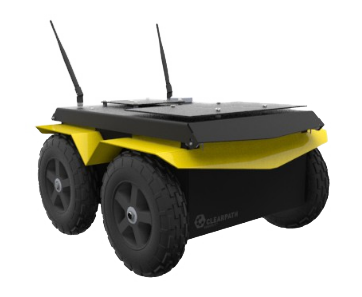
\includegraphics[width=\textwidth]{images/jackal.png}
		\subcaption{Plataforma móvel.}
		\label{fig:pocplat}
	\end{minipage}
	\hfill
	\begin{minipage}[b]{.45\linewidth}
		%		\centering
		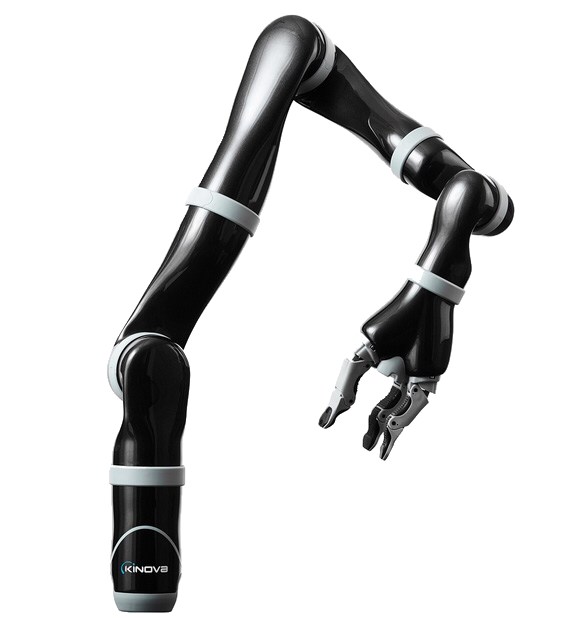
\includegraphics[width=\textwidth]{images/jaco2.png}
		\subcaption{Manipulador.}
		\label{fig:pocmani}
	\end{minipage}
%	\hfill
%	\begin{subfigure}[t]{.3\textwidth}
%		%		\centering
%		\includegraphics[width=\textwidth]{images/whitemarkers.png}
%		\subcaption{Marcadores.}
%		\label{fig:whitemarkers}
%	\end{subfigure}    
	\label{fig:poc}
	\caption{Elementos para a prova de conceito do projeto.}
%	\legend{Fonte: Própria.}
\end{figure}

Dessa forma, esta prova de conceito, subsidiará a análise de viabilidade técnica-econômica prevista para a finalização deste projeto, e que é fundamental para a contratação de futuras fases do projeto.

Além do objetivo principal descrito acima, alguns objetivos específicos devem ser perseguidos para que a conclusão do principal seja alcançada, de forma suscinta é listado estes objetivos específicos:
\begin{itemize}
	\item Projetar e construir a prova de conceito para operação automática de um manipulador 6 \acs{DoF} tendo uma plataforma móvel como referência.
	\item Detalhar operações mais usuais de ROVs e quais manipuladores são utilizados em cada operação.
	\item Elaborar o \textit{\acs{SOTA}} para operação automática de manipuladores submarinos.
	\item Avaliar o custo da operação dos manipuladores e os impactos sobre os custos totais da operação com \acs{ROV}, a partir de referências fornecidas pela PETROBRAS.
	\item Estimar redução nos custos de operação mediante a automatização dos manipuladores, a partir de referências fornecidas pela PETROBRAS.
	\item Elaborar análise de viabilidade técnico-econômica da automatização de operações com manipuladores de \acs{ROV}, a partir de referências fornecidas pela PETROBRAS.
	\item Elaborar um plano de trabalho, considerando que a análise de viabilidade seja positiva, para continuidade do desenvolvimento.
\end{itemize}

No momento atual, alguns desses objetivos já estão sendo desenvolvidos, enquanto outros ainda não foram iniciados; porém espera-se dar início a todos estes objetivos específicos assim que o primeiro workshop seja realizado com o time da Petrobras, que ocorrerá ainda neste mês de maio de 2019.

%---- fase conceitual ------------------------------------
\section{Justificativa}
\label{sec:just}
Nesta etapa da automação de um manipulador, que precede a construção de um protótipo viável em fases futuras, provas de conceito (\textit{\acs{PoC}}) devem ser realizadas em proporções reduzidas em relação às condições reais e em ambiente terrestre, pois acelera o desenvolvimento e possibilita análises de variáveis que podem ser melhor consideradas quando da realização de testes em ambiente controlado. Para isto, algumas abordagens para reproduzir as condições de manipulação subaquática serão testadas demonstrando a aplicação de um ou mais conceitos a partir de diferentes plataformas de desenvolvimento robótico, assim como ferramentas, frameworks, sensores e atuadores que suportem a implementação de técnicas de modelagem de sistemas, controle de posição e de trajetória, integração de sistemas e visão computacional.
A simulação de cenários nas diversas provas de conceitos deverá validar operações que futuramente poderão ser automatizadas por manipuladores subaquáticos em ROVs em intervenções operacionais nas instalações da Petrobrás. 

Um dos pontos importantes na automação de um manipulador robótico é a sua consistência na movimentação de objetos em seu \textit{end-effector}, o fato do desenvolvimento do projeto estar sendo submetido a um ambiente subaquático eleva ainda mais a importância no desenvolvimento de testes conceituais antes da realização do teste final da prova de conceito, onde vários componentes são integrados entre si e desempenham funcionalidades específicas para um ambiente controlado. Trazer estes aspectos para o laboratório é algo que deve ser preponderante para a realização do projeto, pois o mesmo deve ser testado e simulado com elementos capazes de ambientalizar o fenômeno do ponto de visto de controle num ambiente subaquático.

O uso de manipuladores como o sugerido será capaz de trazer à luz do desenvolvimento compreensão sobre as variáveis influenciadoras do evento, utilizados na customização das características técnicas do manipulador robótico a ser testado, os mesmos serão capazes de integrar de forma mais rápida algoritmos a serem desenvolvidos pela equipe do projeto, levando a uma otimização do tempo de desenvolvimento e aumentando a confiabilidade na implementação de controles mais precisos e estáveis.

Dessa forma, a prova de conceito subsidiará a análise de viabilidade técnica-econômica prevista nesta fase, fundamental para a contratação de futuras fases do projeto.

%=========================================================

\section{Organização do relatório}
\label{sec:org}
Este documento está organizado da seguinte forma, o capítulo \ref{chap:int} traz referências iniciais do objetivo deste projeto, o capítulo \ref{chap:robaqua} caracteriza o entendimento sobre a robótica submarina e a atuação dos manipuladores subaquáticos, apresentando de forma suscinta o estado da arte atual para estes elementos, assim como uma pesquisa de anterioridade elaborada para este projeto. O capítulo \ref{chap:manisub-s} descreve a ideia central com relação a prova de conceito que será desenvolvida ao longo deste projeto, chegando a apresentar aspectos iniciais da simulação da prova de conceito. Finalmente, o capítulo \ref{chap:concl} descreve os aspectos conclusivos para esta etapa do projeto.
